This section is going to describe the possible design patterns, which is available to structure our system, implement a user interface, and eventually help simplify the testing process.

\subsubsection{MVC}

MVC stands for Model-View-Controller. The MVC pattern separates the application into three main components: Model, View, and Controller. The model manages the data of the application and responds to requests about its state, usually from the view through an event or the controller.  It also responds to instructions to change state, which is issued by the view, but is performed through the controller. The view displays the state of the model through the graphical user interface, which is received through the controllers, or indirectly by the model. \cite{Pattern1}

\subsubsection{MVVM}

Another pattern that was considered for this project was the MVVM pattern, which is a abbreviation for Model-View-Viewmodel which are the three main components of the pattern. Like MVC, MVVM separates the system into three different components creating a layered structure. The difference between them is that MVVM is much more strict in this separation, which limits the model component to simply containing information about objects, and the view to simply provide a user interface. \cite{Pattern2}

The viewmodel is the component which implements most of the logical code, and is the binding point between the model and the view. The viewmodel implements commands and restrictions, e.g. that binds to a button on the view, and take over the moment a user pushes the button. Beyond the button click, the view gives full control over to the viewmodel. The viewmodel also implements restrictions on the underlying model, so the properties and logic a model normally would have is located in the viewmodel instead. \cite{Pattern2}

\subsubsection{Comparison}

Both patterns provide a layered structure, which can help with testing the system later on, since it is divided into workable parts following these patterns. For this project, the MVC pattern will be used, because it is the more simple of the two patterns and still provides a good testing structure, despite being more loose than the MVVM pattern. MVVM also requires more graphical design, since the view cannot have any notable code-behind. The technicalities behind graphical design is not part of this projects mains goals and is another reason for why MVC was chosen. The MVVM pattern is also better suited for regular desktop applications and since one of the goals is to produce af web application, MVC was again weighed higher than MVVM.

\subsection{Implementation}

\begin{figure}[htb]
\centering
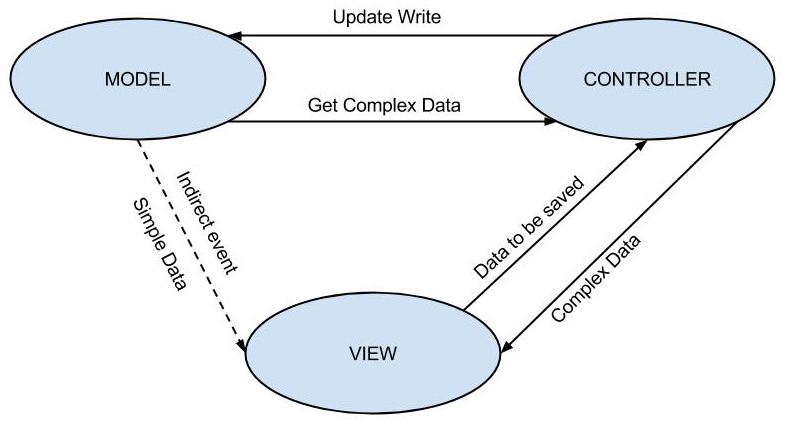
\includegraphics[width=1\textwidth]{Images/MVC.jpg}
\caption{How the MVC is planned to be implemented in this project}
\label{MVC}
\end{figure}

In Figure \ref{MVC} is a representation of how the MVC pattern is planned to be structured in our web application.

The model is the part of the MVC pattern which contains the class structure of the system, describing the classes and their objects. Besides storing class and object information, and communicating with other model members, the model component does not do much on its own and is largely oblivious to the surrounding structure.

The controller is the part of the MVC pattern which processes information it receives from the view and the model, and performs most of the "hard work" in the pattern. Its task changes depending on if it received information from the view or the model and returns something to be shown on the view or something to be stored in the model. This means the controller is the brain of the MVC pattern, and is the binding point between the view and the model.

The view is the part of the MVC pattern that basically is everything visually you can see. What is viewed is usually the classes and objects the model contains, which has been translated to a more understandable format in the GUI, which the user then can see and manipulate. Any changes the user performs goes through the controller, and down into the model. The view is just as “blind” as the model, as it cannot do much on its own, and depends on the controller, and events.

The whole point of using the MVC pattern is to create a layered system, dividing the responsibilities into several components. The MVC pattern can be done in numerious ways, for many different purposes, but this specific pattern is what we found the most appealing for this system. It places the largest need for testing onto the controllers, which contains most of the logical information processing, and the recommendation algorithm. While the GUI is not completely interchangeable like it would be with the MVVM pattern, it is still easier to experiment and further develop with, than without the MVC pattern.